\documentclass[]{article}
\usepackage{lmodern}
\usepackage{amssymb,amsmath}
\usepackage{ifxetex,ifluatex}
\usepackage{fixltx2e} % provides \textsubscript
\ifnum 0\ifxetex 1\fi\ifluatex 1\fi=0 % if pdftex
  \usepackage[T1]{fontenc}
  \usepackage[utf8]{inputenc}
\else % if luatex or xelatex
  \ifxetex
    \usepackage{mathspec}
    \usepackage{xltxtra,xunicode}
  \else
    \usepackage{fontspec}
  \fi
  \defaultfontfeatures{Mapping=tex-text,Scale=MatchLowercase}
  \newcommand{\euro}{€}
\fi
% use upquote if available, for straight quotes in verbatim environments
\IfFileExists{upquote.sty}{\usepackage{upquote}}{}
% use microtype if available
\IfFileExists{microtype.sty}{%
\usepackage{microtype}
\UseMicrotypeSet[protrusion]{basicmath} % disable protrusion for tt fonts
}{}
\usepackage[margin=1in]{geometry}
\ifxetex
  \usepackage[setpagesize=false, % page size defined by xetex
              unicode=false, % unicode breaks when used with xetex
              xetex]{hyperref}
\else
  \usepackage[unicode=true]{hyperref}
\fi
\hypersetup{breaklinks=true,
            bookmarks=true,
            pdfauthor={Zhen Zhang},
            pdftitle={STA141 Assignment 5},
            colorlinks=true,
            citecolor=blue,
            urlcolor=blue,
            linkcolor=magenta,
            pdfborder={0 0 0}}
\urlstyle{same}  % don't use monospace font for urls
\usepackage{color}
\usepackage{fancyvrb}
\newcommand{\VerbBar}{|}
\newcommand{\VERB}{\Verb[commandchars=\\\{\}]}
\DefineVerbatimEnvironment{Highlighting}{Verbatim}{commandchars=\\\{\}}
% Add ',fontsize=\small' for more characters per line
\usepackage{framed}
\definecolor{shadecolor}{RGB}{248,248,248}
\newenvironment{Shaded}{\begin{snugshade}}{\end{snugshade}}
\newcommand{\KeywordTok}[1]{\textcolor[rgb]{0.13,0.29,0.53}{\textbf{{#1}}}}
\newcommand{\DataTypeTok}[1]{\textcolor[rgb]{0.13,0.29,0.53}{{#1}}}
\newcommand{\DecValTok}[1]{\textcolor[rgb]{0.00,0.00,0.81}{{#1}}}
\newcommand{\BaseNTok}[1]{\textcolor[rgb]{0.00,0.00,0.81}{{#1}}}
\newcommand{\FloatTok}[1]{\textcolor[rgb]{0.00,0.00,0.81}{{#1}}}
\newcommand{\ConstantTok}[1]{\textcolor[rgb]{0.00,0.00,0.00}{{#1}}}
\newcommand{\CharTok}[1]{\textcolor[rgb]{0.31,0.60,0.02}{{#1}}}
\newcommand{\SpecialCharTok}[1]{\textcolor[rgb]{0.00,0.00,0.00}{{#1}}}
\newcommand{\StringTok}[1]{\textcolor[rgb]{0.31,0.60,0.02}{{#1}}}
\newcommand{\VerbatimStringTok}[1]{\textcolor[rgb]{0.31,0.60,0.02}{{#1}}}
\newcommand{\SpecialStringTok}[1]{\textcolor[rgb]{0.31,0.60,0.02}{{#1}}}
\newcommand{\ImportTok}[1]{{#1}}
\newcommand{\CommentTok}[1]{\textcolor[rgb]{0.56,0.35,0.01}{\textit{{#1}}}}
\newcommand{\DocumentationTok}[1]{\textcolor[rgb]{0.56,0.35,0.01}{\textbf{\textit{{#1}}}}}
\newcommand{\AnnotationTok}[1]{\textcolor[rgb]{0.56,0.35,0.01}{\textbf{\textit{{#1}}}}}
\newcommand{\CommentVarTok}[1]{\textcolor[rgb]{0.56,0.35,0.01}{\textbf{\textit{{#1}}}}}
\newcommand{\OtherTok}[1]{\textcolor[rgb]{0.56,0.35,0.01}{{#1}}}
\newcommand{\FunctionTok}[1]{\textcolor[rgb]{0.00,0.00,0.00}{{#1}}}
\newcommand{\VariableTok}[1]{\textcolor[rgb]{0.00,0.00,0.00}{{#1}}}
\newcommand{\ControlFlowTok}[1]{\textcolor[rgb]{0.13,0.29,0.53}{\textbf{{#1}}}}
\newcommand{\OperatorTok}[1]{\textcolor[rgb]{0.81,0.36,0.00}{\textbf{{#1}}}}
\newcommand{\BuiltInTok}[1]{{#1}}
\newcommand{\ExtensionTok}[1]{{#1}}
\newcommand{\PreprocessorTok}[1]{\textcolor[rgb]{0.56,0.35,0.01}{\textit{{#1}}}}
\newcommand{\AttributeTok}[1]{\textcolor[rgb]{0.77,0.63,0.00}{{#1}}}
\newcommand{\RegionMarkerTok}[1]{{#1}}
\newcommand{\InformationTok}[1]{\textcolor[rgb]{0.56,0.35,0.01}{\textbf{\textit{{#1}}}}}
\newcommand{\WarningTok}[1]{\textcolor[rgb]{0.56,0.35,0.01}{\textbf{\textit{{#1}}}}}
\newcommand{\AlertTok}[1]{\textcolor[rgb]{0.94,0.16,0.16}{{#1}}}
\newcommand{\ErrorTok}[1]{\textcolor[rgb]{0.64,0.00,0.00}{\textbf{{#1}}}}
\newcommand{\NormalTok}[1]{{#1}}
\usepackage{graphicx,grffile}
\makeatletter
\def\maxwidth{\ifdim\Gin@nat@width>\linewidth\linewidth\else\Gin@nat@width\fi}
\def\maxheight{\ifdim\Gin@nat@height>\textheight\textheight\else\Gin@nat@height\fi}
\makeatother
% Scale images if necessary, so that they will not overflow the page
% margins by default, and it is still possible to overwrite the defaults
% using explicit options in \includegraphics[width, height, ...]{}
\setkeys{Gin}{width=\maxwidth,height=\maxheight,keepaspectratio}
\setlength{\parindent}{0pt}
\setlength{\parskip}{6pt plus 2pt minus 1pt}
\setlength{\emergencystretch}{3em}  % prevent overfull lines
\providecommand{\tightlist}{%
  \setlength{\itemsep}{0pt}\setlength{\parskip}{0pt}}
\setcounter{secnumdepth}{0}

%%% Use protect on footnotes to avoid problems with footnotes in titles
\let\rmarkdownfootnote\footnote%
\def\footnote{\protect\rmarkdownfootnote}

%%% Change title format to be more compact
\usepackage{titling}

% Create subtitle command for use in maketitle
\newcommand{\subtitle}[1]{
  \posttitle{
    \begin{center}\large#1\end{center}
    }
}

\setlength{\droptitle}{-2em}
  \title{STA141 Assignment 5}
  \pretitle{\vspace{\droptitle}\centering\huge}
  \posttitle{\par}
  \author{Zhen Zhang}
  \preauthor{\centering\large\emph}
  \postauthor{\par}
  \predate{\centering\large\emph}
  \postdate{\par}
  \date{November 30, 2015}


% Redefines (sub)paragraphs to behave more like sections
\ifx\paragraph\undefined\else
\let\oldparagraph\paragraph
\renewcommand{\paragraph}[1]{\oldparagraph{#1}\mbox{}}
\fi
\ifx\subparagraph\undefined\else
\let\oldsubparagraph\subparagraph
\renewcommand{\subparagraph}[1]{\oldsubparagraph{#1}\mbox{}}
\fi

\begin{document}
\maketitle

I did this assignment by myself and developed and wrote the code for
each part by myself, drawing only from class, section, Piazza posts and
the Web. I did not use code from a fellow student or a tutor or any
other individual.

\begin{Shaded}
\begin{Highlighting}[]
\KeywordTok{library}\NormalTok{(RSQLite)}
\end{Highlighting}
\end{Shaded}

\begin{verbatim}
## Loading required package: DBI
\end{verbatim}

\begin{Shaded}
\begin{Highlighting}[]
\KeywordTok{library}\NormalTok{(plyr)}
\CommentTok{# read in two databases}
\NormalTok{con =}\StringTok{ }\KeywordTok{dbConnect}\NormalTok{(}\KeywordTok{SQLite}\NormalTok{(), }\StringTok{'lean_imdbpy.db'}\NormalTok{)}
\NormalTok{con2 =}\StringTok{ }\KeywordTok{dbConnect}\NormalTok{(}\KeywordTok{SQLite}\NormalTok{(), }\StringTok{'lean_imdbpy_2010_idx.db'}\NormalTok{)}
\end{Highlighting}
\end{Shaded}

\subsubsection{1}\label{section}

\begin{Shaded}
\begin{Highlighting}[]
\CommentTok{# number of movies}

\CommentTok{# In this part I will create two new tables, which I will use afterwards all the time.}
\CommentTok{# One is title_movie, which is the subset of title only containing movies. The other is}
\CommentTok{# name_actor, which is also a subset of name only containing actors. Since questions}
\CommentTok{# afterwards will keep focused on movies and actors, I will create them as temporary}
\CommentTok{# tables.}

\CommentTok{# create a new title table that only have movies, and give the table name title_movie}
\CommentTok{# NOTE: THIS WILL BE RUN FOR ONLY ONE TIME SINCE IT WILL CREATE A NEW TABLE}

\CommentTok{# dbGetQuery(con, '}
\CommentTok{#            CREATE TABLE title_movie AS}
\CommentTok{#            SELECT DISTINCT title.*}
\CommentTok{#            FROM title JOIN kind_type kt ON title.kind_id = kt.id}
\CommentTok{#            WHERE kt.kind = "movie"}
\CommentTok{#            ')}

\KeywordTok{dbGetQuery}\NormalTok{(con, }\StringTok{'}
\StringTok{           SELECT COUNT(DISTINCT title_movie.id) movie_count}
\StringTok{           FROM title_movie}
\StringTok{           '}\NormalTok{)}
\end{Highlighting}
\end{Shaded}

\begin{verbatim}
##   movie_count
## 1      878800
\end{verbatim}

\begin{Shaded}
\begin{Highlighting}[]
\CommentTok{# number of actors}

\CommentTok{# create a new name table that only have actors, and give the table name name_actor}
\CommentTok{# Also one table}

\CommentTok{# dbGetQuery(con, '}
\CommentTok{#            CREATE TABLE name_actor AS}
\CommentTok{#            SELECT DISTINCT name.*}
\CommentTok{#            FROM cast_info ci JOIN name ON ci.person_id = name.id}
\CommentTok{#               JOIN role_type rt on ci.role_id = rt.id}
\CommentTok{#            WHERE rt.role IN ("actor", "actress")}
\CommentTok{#            ')}


\KeywordTok{dbGetQuery}\NormalTok{(con, }\StringTok{'}
\StringTok{           SELECT count(name_actor.id) actor_count}
\StringTok{           FROM name_actor}
\StringTok{           '}\NormalTok{)}
\end{Highlighting}
\end{Shaded}

\begin{verbatim}
##   actor_count
## 1     3492018
\end{verbatim}

\subsubsection{2}\label{section}

\begin{Shaded}
\begin{Highlighting}[]
\CommentTok{# year span}
\KeywordTok{dbGetQuery}\NormalTok{(con, }\StringTok{'}
\StringTok{           SELECT MAX(production_year) year_max, MIN(production_year) year_min}
\StringTok{           FROM title}
\StringTok{           '}\NormalTok{)}
\end{Highlighting}
\end{Shaded}

\begin{verbatim}
##   year_max year_min
## 1     2025     1874
\end{verbatim}

\subsubsection{3}\label{section-1}

\begin{Shaded}
\begin{Highlighting}[]
\CommentTok{# get the count of each gender}
\NormalTok{each_gender <-}\StringTok{ }
\StringTok{  }\KeywordTok{dbGetQuery}\NormalTok{(con, }\StringTok{'}
\StringTok{             SELECT COUNT(*) gender_count, gender }
\StringTok{             FROM name_actor}
\StringTok{             GROUP BY gender;}
\StringTok{             '}\NormalTok{)}

\CommentTok{# get the total count}
\NormalTok{total_number_gender <-}\StringTok{ }
\StringTok{  }\KeywordTok{dbGetQuery}\NormalTok{(con, }\StringTok{'}
\StringTok{             SELECT COUNT(*)}
\StringTok{             FROM name_actor}
\StringTok{             '}\NormalTok{)}

\CommentTok{# propotionalized}
\NormalTok{each_gender$gender_count <-}\StringTok{ }\NormalTok{each_gender$gender_count /}\StringTok{ }\NormalTok{total_number_gender[[}\DecValTok{1}\NormalTok{]]}

\CommentTok{# return result}
\NormalTok{each_gender}
\end{Highlighting}
\end{Shaded}

\begin{verbatim}
##   gender_count gender
## 1    0.3537021      f
## 2    0.6462979      m
\end{verbatim}

\subsubsection{4}\label{section-2}

\begin{Shaded}
\begin{Highlighting}[]
\CommentTok{# get the count of type}
\NormalTok{each_kind <-}\StringTok{ }
\StringTok{  }\KeywordTok{dbGetQuery}\NormalTok{(con, }\StringTok{'}
\StringTok{             SELECT COUNT(*) type_count, kt.kind }
\StringTok{             FROM title JOIN kind_type kt ON title.kind_id = kt.id}
\StringTok{             GROUP BY kt.kind}
\StringTok{             '}\NormalTok{)}

\CommentTok{# get the total number}
\NormalTok{total_number_kind <-}\StringTok{ }
\StringTok{  }\KeywordTok{dbGetQuery}\NormalTok{(con, }\StringTok{'}
\StringTok{             SELECT COUNT(*)}
\StringTok{             FROM title}
\StringTok{             '}\NormalTok{)}

\CommentTok{# proportionalize}
\NormalTok{each_kind$type_count <-}\StringTok{ }\NormalTok{each_kind$type_count /}\StringTok{ }\NormalTok{total_number_kind[[}\DecValTok{1}\NormalTok{]]}

\CommentTok{# print result}
\NormalTok{each_kind}
\end{Highlighting}
\end{Shaded}

\begin{verbatim}
##    type_count        kind
## 1 0.635583712     episode
## 2 0.249111894       movie
## 3 0.034126175    tv movie
## 4 0.035273371   tv series
## 5 0.004341033  video game
## 6 0.041563815 video movie
\end{verbatim}

\subsubsection{5}\label{section}

\begin{Shaded}
\begin{Highlighting}[]
\CommentTok{# get the number of genres}
\KeywordTok{dbGetQuery}\NormalTok{(con, }\StringTok{'}
\StringTok{           SELECT COUNT(*) genre_count}
\StringTok{           FROM (}
\StringTok{              SELECT mi.info}
\StringTok{              FROM info_type it JOIN movie_info mi ON it.id = mi.info_type_id}
\StringTok{                  JOIN title_movie tm ON mi.movie_id = tm.id}
\StringTok{              WHERE it.info = "genres"}
\StringTok{              GROUP BY mi.info}
\StringTok{           )}
\StringTok{           '}\NormalTok{)}
\end{Highlighting}
\end{Shaded}

\begin{verbatim}
##   genre_count
## 1          28
\end{verbatim}

\begin{Shaded}
\begin{Highlighting}[]
\CommentTok{# get all genres}
\KeywordTok{dbGetQuery}\NormalTok{(con, }\StringTok{'}
\StringTok{           SELECT mi.info}
\StringTok{           FROM info_type it INNER JOIN movie_info mi ON it.id = mi.info_type_id}
\StringTok{              INNER JOIN title_movie tm ON mi.movie_id = tm.id}
\StringTok{           WHERE it.info = "genres"}
\StringTok{           GROUP BY mi.info}
\StringTok{           '}\NormalTok{)}
\end{Highlighting}
\end{Shaded}

\begin{verbatim}
##           info
## 1       Action
## 2        Adult
## 3    Adventure
## 4    Animation
## 5    Biography
## 6       Comedy
## 7        Crime
## 8  Documentary
## 9        Drama
## 10      Family
## 11     Fantasy
## 12   Film-Noir
## 13   Game-Show
## 14     History
## 15      Horror
## 16       Music
## 17     Musical
## 18     Mystery
## 19        News
## 20  Reality-TV
## 21     Romance
## 22      Sci-Fi
## 23       Short
## 24       Sport
## 25   Talk-Show
## 26    Thriller
## 27         War
## 28     Western
\end{verbatim}

\begin{Shaded}
\begin{Highlighting}[]
\CommentTok{# What if we want genres from all movies and tvs and others?}
\KeywordTok{dbGetQuery}\NormalTok{(con, }\StringTok{'}
\StringTok{           SELECT mi.info}
\StringTok{           FROM info_type it INNER JOIN movie_info mi ON it.id = mi.info_type_id}
\StringTok{              INNER JOIN title tm ON mi.movie_id = tm.id}
\StringTok{           WHERE it.info = "genres"}
\StringTok{           GROUP BY mi.info}
\StringTok{           '}\NormalTok{)}
\end{Highlighting}
\end{Shaded}

\begin{verbatim}
##            info
## 1        Action
## 2         Adult
## 3     Adventure
## 4     Animation
## 5     Biography
## 6        Comedy
## 7    Commercial
## 8         Crime
## 9   Documentary
## 10        Drama
## 11      Erotica
## 12 Experimental
## 13       Family
## 14      Fantasy
## 15    Film-Noir
## 16    Game-Show
## 17      History
## 18       Horror
## 19    Lifestyle
## 20        Music
## 21      Musical
## 22      Mystery
## 23         News
## 24   Reality-TV
## 25      Romance
## 26       Sci-Fi
## 27        Short
## 28        Sport
## 29    Talk-Show
## 30     Thriller
## 31          War
## 32      Western
\end{verbatim}

\subsubsection{6}\label{section}

\begin{Shaded}
\begin{Highlighting}[]
\CommentTok{# the 10 most common genres of movies, showing the number of movies in each of }
\CommentTok{# these genres}
\NormalTok{top_10_genres <-}\StringTok{ }
\StringTok{  }\KeywordTok{dbGetQuery}\NormalTok{(con, }\StringTok{'}
\StringTok{             SELECT mi.info, COUNT(mi.info) genre_count}
\StringTok{             FROM info_type it INNER JOIN movie_info mi ON it.id = mi.info_type_id}
\StringTok{                INNER JOIN title_movie tm ON mi.movie_id = tm.id}
\StringTok{             WHERE it.info = "genres"}
\StringTok{             GROUP BY mi.info}
\StringTok{             ORDER BY genre_count DESC}
\StringTok{             LIMIT 10}
\StringTok{             '}\NormalTok{)}

\NormalTok{top_10_genres}
\end{Highlighting}
\end{Shaded}

\begin{verbatim}
##           info genre_count
## 1        Short      470488
## 2        Drama      269898
## 3       Comedy      180315
## 4  Documentary      145018
## 5      Romance       52324
## 6     Thriller       51961
## 7       Action       45077
## 8       Horror       38620
## 9    Animation       38461
## 10       Crime       33010
\end{verbatim}

\subsubsection{7}\label{section-1}

\begin{Shaded}
\begin{Highlighting}[]
\CommentTok{# all movies with the keyword 'space'}
\NormalTok{movie_space <-}
\StringTok{  }\KeywordTok{dbGetQuery}\NormalTok{(con, }\StringTok{'}
\StringTok{             SELECT tm.id, tm.title}
\StringTok{             FROM title_movie tm INNER JOIN movie_keyword mk ON tm.id = mk.movie_id}
\StringTok{                INNER JOIN keyword kw ON mk.keyword_id = kw.id}
\StringTok{             WHERE kw.keyword = "space"}
\StringTok{             '}\NormalTok{)}

\KeywordTok{head}\NormalTok{(movie_space)}
\end{Highlighting}
\end{Shaded}

\begin{verbatim}
##        id                        title
## 1 2365979          002 operazione Luna
## 2 2367917               12 to the Moon
## 3 2371167    20 Million Miles to Earth
## 4 2371436        2001: A Space Odyssey
## 5 2371922                         2010
## 6 2376022 4: Rise of the Silver Surfer
\end{verbatim}

\begin{Shaded}
\begin{Highlighting}[]
\KeywordTok{summary}\NormalTok{(movie_space)}
\end{Highlighting}
\end{Shaded}

\begin{verbatim}
##        id             title
##  Min.   :2365979   Length:401
##  1st Qu.:2668393   Class :character
##  Median :3004151   Mode  :character
##  Mean   :2969881
##  3rd Qu.:3241566
##  Max.   :3521673
\end{verbatim}

\begin{Shaded}
\begin{Highlighting}[]
\CommentTok{# count}
\KeywordTok{dbGetQuery}\NormalTok{(con, }\StringTok{'}
\StringTok{           SELECT COUNT(*) space_count}
\StringTok{           FROM title_movie tm INNER JOIN movie_keyword mk ON tm.id = mk.movie_id}
\StringTok{              INNER JOIN keyword kw ON mk.keyword_id = kw.id}
\StringTok{           WHERE kw.keyword = "space"}
\StringTok{           '}\NormalTok{)}
\end{Highlighting}
\end{Shaded}

\begin{verbatim}
##   space_count
## 1         401
\end{verbatim}

\begin{Shaded}
\begin{Highlighting}[]
\CommentTok{# years}
\NormalTok{movie_space_year <-}\StringTok{ }
\StringTok{  }\KeywordTok{dbGetQuery}\NormalTok{(con, }\StringTok{'}
\StringTok{             SELECT DISTINCT tm.production_year}
\StringTok{             FROM title_movie tm INNER JOIN movie_keyword mk ON tm.id = mk.movie_id}
\StringTok{                INNER JOIN keyword kw ON mk.keyword_id = kw.id}
\StringTok{             WHERE kw.keyword = "space" AND tm.production_year IS NOT NULL}
\StringTok{             ORDER BY tm.production_year}
\StringTok{             '}\NormalTok{)}

\NormalTok{movie_space_year$production_year}
\end{Highlighting}
\end{Shaded}

\begin{verbatim}
##  [1] 1911 1918 1922 1925 1930 1946 1947 1950 1951 1953 1954 1955 1956 1957
## [15] 1958 1959 1960 1961 1962 1964 1965 1966 1967 1968 1969 1970 1971 1972
## [29] 1973 1974 1975 1977 1978 1979 1980 1981 1982 1983 1984 1985 1986 1987
## [43] 1988 1989 1990 1991 1992 1993 1994 1996 1997 1998 1999 2000 2001 2002
## [57] 2003 2004 2005 2006 2007 2008 2009 2010 2011 2012 2013 2014 2015 2016
## [71] 2017 2018
\end{verbatim}

\begin{Shaded}
\begin{Highlighting}[]
\CommentTok{# top n actors with each movie}

\NormalTok{movie_space_top_actor_each <-}\StringTok{ }\NormalTok{function(n) \{}
  \CommentTok{# This is the function that gives the result of top 5 movies with n movies. So if}
  \CommentTok{# you want the data for the first 10 movies, just give the argument n = 10, and this}
  \CommentTok{# is what I do afterwards.}

  \NormalTok{top_actor <-}\StringTok{ }\KeywordTok{lapply}\NormalTok{(movie_space[[}\StringTok{'id'}\NormalTok{]][}\DecValTok{1}\NormalTok{:n], function(x) \{}
                \KeywordTok{dbGetQuery}\NormalTok{(con, }\KeywordTok{paste}\NormalTok{(}\StringTok{'}
\StringTok{                           SELECT na.id, na.name, ci.nr_order}
\StringTok{                           FROM title_movie tm JOIN cast_info ci ON tm.id = ci.movie_id}
\StringTok{                              JOIN name_actor na ON na.id = ci.person_id}
\StringTok{                           WHERE tm.id ='}\NormalTok{, x, }\StringTok{'}
\StringTok{                           AND ci.nr_order IN (1, 2, 3, 4, 5, 6)}
\StringTok{                           GROUP BY na.id}
\StringTok{                           ORDER BY ci.nr_order}
\StringTok{                           LIMIT 5'}
                           \NormalTok{))}
              \NormalTok{\})}

  \KeywordTok{names}\NormalTok{(top_actor) <-}\StringTok{ }\NormalTok{movie_space[[}\StringTok{'name'}\NormalTok{]][}\DecValTok{1}\NormalTok{:n]}

  \NormalTok{top_actor}
\NormalTok{\}}

\NormalTok{movie_space_top_actor_total <-}\StringTok{ }\KeywordTok{movie_space_top_actor_each}\NormalTok{(}\DecValTok{10}\NormalTok{)}

\NormalTok{movie_space_top_actor_total}
\end{Highlighting}
\end{Shaded}

\begin{verbatim}
## [[1]]
##        id              name nr_order
## 1  661113   Franchi, Franco        1
## 2  935665 Ingrassia, Ciccio        2
## 3 3172528   Randall, Mónica        3
## 4 3291555       Sini, Linda        4
## 5 3286328      Silva, María        5
##
## [[2]]
##        id            name nr_order
## 1  374630      Clark, Ken        1
## 2 2845023     Kobi, Michi        2
## 3  402504     Conway, Tom        3
## 4  506884 Dexter, Anthony        4
## 5 2164166   Wengraf, John        5
##
## [[3]]
##        id              name nr_order
## 1  899083   Hopper, William        1
## 2 2843284 Knight, Charlotte        1
## 3 3357735      Taylor, Joan        2
## 4 1633148     Puglia, Frank        3
## 5 2243618     Zaremba, John        4
##
## [[4]]
##        id               name nr_order
## 1  550078       Dullea, Keir        1
## 2 1195795     Lockwood, Gary        2
## 3 1974787 Sylvester, William        3
## 4 1694544    Richter, Daniel        4
## 5 1740095  Rossiter, Leonard        5
##
## [[5]]
##        id          name nr_order
## 1  924468  Hyams, Peter        1
## 2 1803971 Scheider, Roy        1
## 3 1189509 Lithgow, John        2
## 4 3016212 Mirren, Helen        3
## 5  111419  Balaban, Bob        4
##
## [[6]]
##        id           name nr_order
## 1  782884 Gruffudd, Ioan        1
## 2 2060367   Turman, John        1
## 3 1155168      Lee, Stan        2
## 4 2275575  Alba, Jessica        2
## 5  599152   Evans, Chris        3
##
## [[7]]
## [1] id       name     nr_order
## <0 rows> (or 0-length row.names)
##
## [[8]]
##        id                   name nr_order
## 1 2122907 von Zeddelmann, Moritz        1
## 2 3098065    Osterloh, Dolly-Ann        2
## 3  425764           Cree, Steven        3
## 4 1440847          Nallon, Steve        4
## 5  539062           Doyle, Jamie        5
##
## [[9]]
## [1] id       name     nr_order
## <0 rows> (or 0-length row.names)
##
## [[10]]
## [1] id       name     nr_order
## <0 rows> (or 0-length row.names)
\end{verbatim}

\subsubsection{8}\label{section}

\begin{Shaded}
\begin{Highlighting}[]
\CommentTok{# The number of genres over time}
\NormalTok{genre_year <-}\StringTok{ }
\StringTok{  }\KeywordTok{dbGetQuery}\NormalTok{(con, }\StringTok{'}
\StringTok{                  SELECT mi.info genre, tm.production_year year, COUNT(mi.info) genre_count}
\StringTok{                  FROM info_type it JOIN movie_info mi ON it.id = mi.info_type_id}
\StringTok{                      JOIN title_movie tm ON mi.movie_id = tm.id}
\StringTok{                  WHERE it.info = "genres" AND }
\StringTok{                      tm.production_year IS NOT NULL AND }
\StringTok{                      genre IS NOT NULL}
\StringTok{                  GROUP BY mi.info, tm.production_year}
\StringTok{                  '}\NormalTok{)}

\KeywordTok{library}\NormalTok{(ggplot2)}

\CommentTok{# here I control the observations to make separate geners on 2 different plots}
\KeywordTok{ggplot}\NormalTok{(genre_year[}\DecValTok{1}\NormalTok{:}\DecValTok{1778}\NormalTok{, ], }\KeywordTok{aes}\NormalTok{(year, genre_count)) +}\StringTok{ }
\StringTok{  }\KeywordTok{geom_point}\NormalTok{() +}\StringTok{ }
\StringTok{  }\KeywordTok{facet_wrap}\NormalTok{(~}\StringTok{ }\NormalTok{genre, }\DataTypeTok{scales =} \StringTok{'free'}\NormalTok{)}
\end{Highlighting}
\end{Shaded}

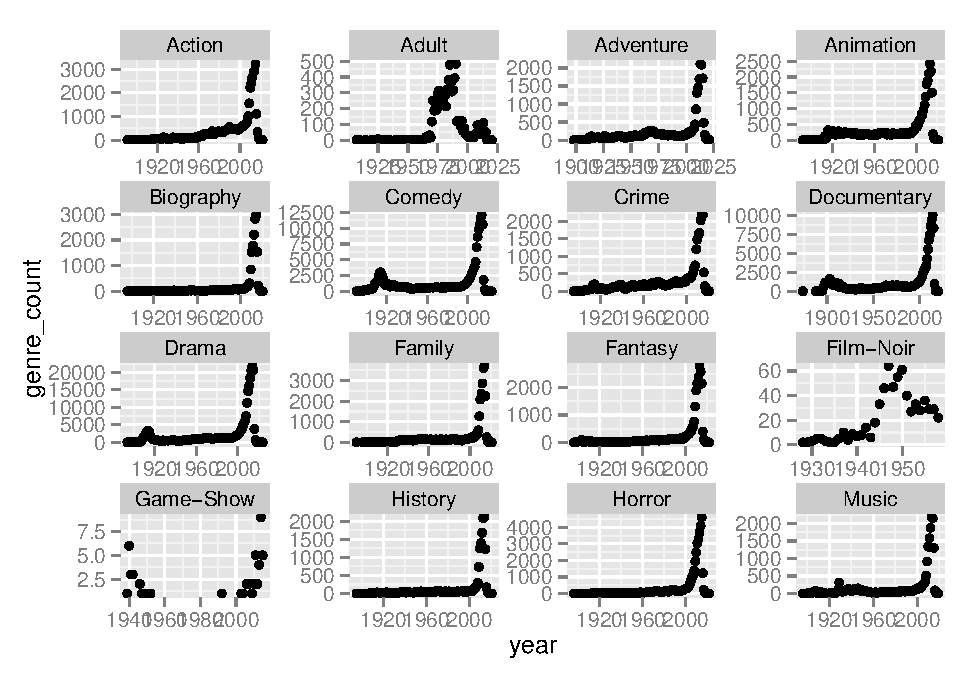
\includegraphics{test2_files/figure-latex/unnamed-chunk-2-1.pdf}

\begin{Shaded}
\begin{Highlighting}[]
\KeywordTok{ggplot}\NormalTok{(genre_year[}\DecValTok{1779}\NormalTok{:}\KeywordTok{dim}\NormalTok{(genre_year)[}\DecValTok{1}\NormalTok{], ], }\KeywordTok{aes}\NormalTok{(year, genre_count)) +}\StringTok{ }
\StringTok{  }\KeywordTok{geom_point}\NormalTok{() +}\StringTok{ }
\StringTok{  }\KeywordTok{facet_wrap}\NormalTok{(~}\StringTok{ }\NormalTok{genre, }\DataTypeTok{scales =} \StringTok{'free'}\NormalTok{)}
\end{Highlighting}
\end{Shaded}

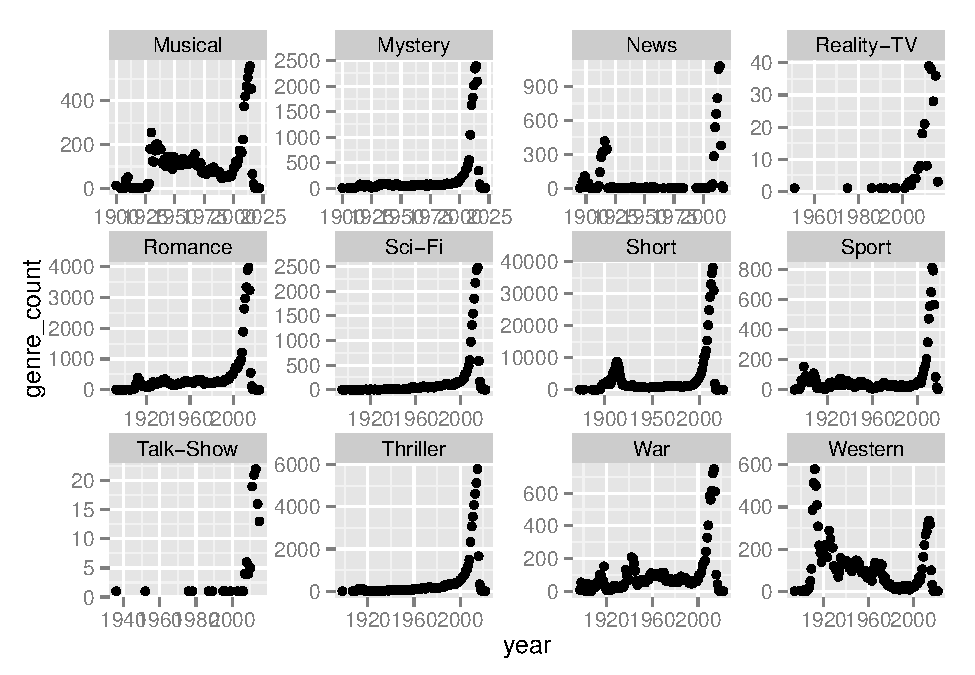
\includegraphics{test2_files/figure-latex/unnamed-chunk-2-2.pdf}

\begin{Shaded}
\begin{Highlighting}[]
\CommentTok{# From the figure I can see that, most of the movies increase the number after year 2000}
\CommentTok{# rapidly, except movie genre western and war.}
\end{Highlighting}
\end{Shaded}

\subsubsection{9-12 are using small dataset}\label{are-using-small-dataset}

\begin{Shaded}
\begin{Highlighting}[]
\CommentTok{# To be consistent, I will also create two tables as before, which are movies and actors}
\CommentTok{# THIS WILL BE DONE ONLY ONCE}

\CommentTok{# dbGetQuery(con2, '}
\CommentTok{#            CREATE TABLE title_movie2 AS}
\CommentTok{#            SELECT DISTINCT title2.*}
\CommentTok{#            FROM title2 JOIN kind_type kt ON title2.kind_id = kt.id}
\CommentTok{#            WHERE kt.kind = "movie"}
\CommentTok{#            ')}
\CommentTok{# }
\CommentTok{# dbGetQuery(con2, '}
\CommentTok{#            CREATE TABLE name_actor2 AS}
\CommentTok{#            SELECT DISTINCT name2.*}
\CommentTok{#            FROM cast_info2 ci JOIN name2 ON ci.person_id = name2.id}
\CommentTok{#            JOIN role_type rt on ci.role_id = rt.id}
\CommentTok{#            WHERE rt.role IN ("actor", "actress")}
\CommentTok{#            ')}
\end{Highlighting}
\end{Shaded}

\begin{Shaded}
\begin{Highlighting}[]
\CommentTok{# Here I will first get all tables I need from sql and then join them}

\CommentTok{# name_actor}
\NormalTok{data_na <-}\StringTok{ }
\StringTok{  }\KeywordTok{dbGetQuery}\NormalTok{(con2, }\StringTok{'}
\StringTok{                   SELECT *}
\StringTok{                   FROM name_actor2 na}
\StringTok{                   '}\NormalTok{)}
\KeywordTok{names}\NormalTok{(data_na) <-}\StringTok{ }\KeywordTok{paste0}\NormalTok{(}\StringTok{'na.'}\NormalTok{,}\KeywordTok{names}\NormalTok{(data_na))}

\CommentTok{# title_movie}
\NormalTok{data_tm <-}\StringTok{ }
\StringTok{  }\KeywordTok{dbGetQuery}\NormalTok{(con2, }\StringTok{'}
\StringTok{             SELECT *}
\StringTok{             FROM title_movie2 tm}
\StringTok{             '}\NormalTok{)}
\KeywordTok{names}\NormalTok{(data_tm) <-}\StringTok{ }\KeywordTok{paste0}\NormalTok{(}\StringTok{'tm.'}\NormalTok{,}\KeywordTok{names}\NormalTok{(data_tm))}

\CommentTok{# cast_info}
\NormalTok{data_ci <-}\StringTok{ }
\StringTok{  }\KeywordTok{dbGetQuery}\NormalTok{(con2, }\StringTok{'}
\StringTok{             SELECT *}
\StringTok{             FROM cast_info2 ci}
\StringTok{             '}\NormalTok{)}
\KeywordTok{names}\NormalTok{(data_ci) <-}\StringTok{ }\KeywordTok{paste0}\NormalTok{(}\StringTok{'ci.'}\NormalTok{,}\KeywordTok{names}\NormalTok{(data_ci))}

\CommentTok{# inner join them, use package dplyr}
\KeywordTok{library}\NormalTok{(dplyr)}

\NormalTok{data_na_tm_ci <-}\StringTok{ }
\StringTok{  }\KeywordTok{inner_join}\NormalTok{(}
    \KeywordTok{inner_join}\NormalTok{(}
      \NormalTok{data_na, data_ci, }\DataTypeTok{by =} \KeywordTok{c}\NormalTok{(}\StringTok{'na.id'} \NormalTok{=}\StringTok{ 'ci.person_id'}\NormalTok{)}
      \NormalTok{), }
    \NormalTok{data_tm, }\DataTypeTok{by =} \KeywordTok{c}\NormalTok{(}\StringTok{'ci.movie_id'} \NormalTok{=}\StringTok{ 'tm.id'}\NormalTok{)}
    \NormalTok{)}

\CommentTok{# Then when I am using R, I can just select columns in data_na_tm_ci}
\end{Highlighting}
\end{Shaded}

\subsubsection{9}\label{section-1}

\begin{Shaded}
\begin{Highlighting}[]
\CommentTok{# Top 20 actors in movies}

\CommentTok{# SQL approach}
\KeywordTok{dbGetQuery}\NormalTok{(con2, }\StringTok{'}
\StringTok{           SELECT na.id, na.name, COUNT(*) actor_count}
\StringTok{           FROM cast_info2 ci JOIN name_actor2 na ON ci.person_id = na.id}
\StringTok{              JOIN title_movie2 tm ON tm.id = ci.movie_id}
\StringTok{           GROUP BY na.id}
\StringTok{           ORDER BY actor_count DESC}
\StringTok{           LIMIT 20}
\StringTok{           '}\NormalTok{)}
\end{Highlighting}
\end{Shaded}

\begin{verbatim}
##         id                   name actor_count
## 1  1234086         MacLeod, Kevin        1508
## 2   568207           Edward, Noah         625
## 3  1705106          Rivers, Scott         529
## 4   636012 Fischbach, Mark Edward         443
## 5   919340             Hunter, G.         381
## 6  1228623          Macaroni, Sam         380
## 7  1735527           Rosen, Larry         340
## 8  1459666          Newton, Brett         339
## 9  1549168            Pasha, Omer         332
## 10 1217855            Lund, Tyler         329
## 11 1887456          Sloan, Lee A.         311
## 12  430358           Cross, Logan         294
## 13 2228101      Yeriomin, Nikolay         267
## 14 1819953         Sciolè, Flavio         246
## 15 1479028     Notarile, Chris R.         244
## 16 1366507          Mills, Travis         239
## 17     686             A., Sergey         236
## 18 2156581            Weecks, Dan         228
## 19 1488023       O'Connor, George         225
## 20 1700138       Ringgaard, Peter         214
\end{verbatim}

\begin{Shaded}
\begin{Highlighting}[]
\CommentTok{# R approach}

\CommentTok{# extract data}
\NormalTok{actors <-}\StringTok{ }\NormalTok{data_na_tm_ci[, }\KeywordTok{c}\NormalTok{(}\StringTok{'na.id'}\NormalTok{, }\StringTok{'na.name'}\NormalTok{)]}
\KeywordTok{names}\NormalTok{(actors) <-}\StringTok{ }\KeywordTok{c}\NormalTok{(}\StringTok{'id'}\NormalTok{, }\StringTok{'name'}\NormalTok{)}

\CommentTok{# use ddply to first split data by id and name, then count the number}
\NormalTok{actors_count <-}\StringTok{ }\KeywordTok{ddply}\NormalTok{(actors, .(id, name), nrow)}

\CommentTok{# see the top 20}
\KeywordTok{head}\NormalTok{(actors_count[}\KeywordTok{order}\NormalTok{(actors_count$V1, }\DataTypeTok{decreasing =} \NormalTok{T), ], }\DataTypeTok{n =} \DecValTok{20}\NormalTok{)}
\end{Highlighting}
\end{Shaded}

\begin{verbatim}
##             id                   name   V1
## 412384 1234086         MacLeod, Kevin 1508
## 191576  568207           Edward, Noah  625
## 571846 1705106          Rivers, Scott  529
## 214117  636012 Fischbach, Mark Edward  443
## 309021  919340             Hunter, G.  381
## 410604 1228623          Macaroni, Sam  380
## 582261 1735527           Rosen, Larry  340
## 489611 1459666          Newton, Brett  339
## 519791 1549168            Pasha, Omer  332
## 407229 1217855            Lund, Tyler  329
## 633089 1887456          Sloan, Lee A.  311
## 145976  430358           Cross, Logan  294
## 745514 2228101      Yeriomin, Nikolay  267
## 610069 1819953         Sciolè, Flavio  246
## 496066 1479028     Notarile, Chris R.  244
## 458089 1366507          Mills, Travis  239
## 231        686             A., Sergey  236
## 721032 2156581            Weecks, Dan  228
## 499050 1488023       O'Connor, George  225
## 570129 1700138       Ringgaard, Peter  214
\end{verbatim}

\subsubsection{10}\label{section}

\begin{Shaded}
\begin{Highlighting}[]
\CommentTok{# top billing}

\CommentTok{# SQL approach}
\NormalTok{billing_top_10 <-}\StringTok{ }
\StringTok{  }\KeywordTok{dbGetQuery}\NormalTok{(con2, }\StringTok{'}
\StringTok{             SELECT na.id, na.name, COUNT(na.id) actor_billing_count, }
\StringTok{                MIN(tm.production_year) min_year, MAX(tm.production_year) max_year}
\StringTok{             FROM name_actor2 na JOIN cast_info2 ci on na.id = ci.person_id}
\StringTok{                JOIN title_movie2 tm ON tm.id = ci.movie_id}
\StringTok{             WHERE ci.nr_order IN (1, 2, 3)}
\StringTok{             GROUP BY na.id}
\StringTok{             ORDER BY COUNT(na.id) DESC}
\StringTok{             LIMIT 10}
\StringTok{             '}\NormalTok{)}

\NormalTok{billing_top_10}
\end{Highlighting}
\end{Shaded}

\begin{verbatim}
##         id                      name actor_billing_count min_year max_year
## 1  1204854            Lorente, Txema                 106     2010     2015
## 2  1708783             Roberts, Eric                  75     2010     2016
## 3  1881637             Sizemore, Tom                  48     2010     2016
## 4  1488023          O'Connor, George                  46     2014     2015
## 5  2046271              Trejo, Danny                  43     2010     2015
## 6   292687 Calderón, Emilio Janhunen                  38     2011     2015
## 7   257734            Brown, Shannon                  37     2011     2016
## 8  1302470         Mazak, Kasey Ryne                  37     2010     2015
## 9  1237239           Madsen, Michael                  35     2010     2016
## 10 1381086                  Mohanlal                  34     2010     2015
\end{verbatim}

\begin{Shaded}
\begin{Highlighting}[]
\CommentTok{# R approach}

\CommentTok{# extract data}
\NormalTok{billing_data <-}\StringTok{ }\NormalTok{data_na_tm_ci[, }\KeywordTok{c}\NormalTok{(}\StringTok{'na.id'}\NormalTok{, }\StringTok{'na.name'}\NormalTok{, }\StringTok{'tm.production_year'}\NormalTok{, }\StringTok{'ci.nr_order'}\NormalTok{)]}
\KeywordTok{names}\NormalTok{(billing_data) <-}\StringTok{ }\KeywordTok{c}\NormalTok{(}\StringTok{'id'}\NormalTok{, }\StringTok{'name'}\NormalTok{, }\StringTok{'production_year'}\NormalTok{, }\StringTok{'nr_order'}\NormalTok{)}

\CommentTok{# subset by only nr_order of 1, 2, 3, and for columns, drop the nr_order}
\NormalTok{billing_top_data <-}\StringTok{ }\NormalTok{billing_data[billing_data$nr_order %in%}\StringTok{ }\KeywordTok{c}\NormalTok{(}\DecValTok{1}\NormalTok{, }\DecValTok{2}\NormalTok{, }\DecValTok{3}\NormalTok{), -}\DecValTok{4}\NormalTok{]}

\CommentTok{# use ddply to split id and name, and count the number and the corresponding year span}
\NormalTok{billing_top_data_count <-}\StringTok{ }\KeywordTok{ddply}\NormalTok{(billing_top_data, .(id, name), nrow)}

\CommentTok{# get the top 10 movies}
\NormalTok{billing_top_data_count_head <-}\StringTok{ }
\StringTok{  }\KeywordTok{head}\NormalTok{(billing_top_data_count[}\KeywordTok{order}\NormalTok{(billing_top_data_count$V1, }\DataTypeTok{decreasing =} \NormalTok{T), ], }\DataTypeTok{n =} \DecValTok{10}\NormalTok{)}
\CommentTok{# get the max and min year}
\NormalTok{billing_top_data_count_head$max_year <-}\StringTok{ }
\StringTok{  }\KeywordTok{sapply}\NormalTok{(}\DecValTok{1}\NormalTok{:}\KeywordTok{nrow}\NormalTok{(billing_top_data_count_head), function(i) \{}
    \KeywordTok{max}\NormalTok{(billing_data[billing_data$id ==}\StringTok{ }\NormalTok{billing_top_data_count_head[i, }\StringTok{'id'}\NormalTok{], }\StringTok{'production_year'}\NormalTok{])}
  \NormalTok{\})}
\NormalTok{billing_top_data_count_head$min_year <-}\StringTok{ }
\StringTok{  }\KeywordTok{sapply}\NormalTok{(}\DecValTok{1}\NormalTok{:}\KeywordTok{nrow}\NormalTok{(billing_top_data_count_head), function(i) \{}
    \KeywordTok{min}\NormalTok{(billing_data[billing_data$id ==}\StringTok{ }\NormalTok{billing_top_data_count_head[i, }\StringTok{'id'}\NormalTok{], }\StringTok{'production_year'}\NormalTok{])}
  \NormalTok{\})}

\NormalTok{billing_top_data_count_head}
\end{Highlighting}
\end{Shaded}

\begin{verbatim}
##            id                      name  V1 max_year min_year
## 44049 1204854            Lorente, Txema 106     2015     2010
## 62242 1708783             Roberts, Eric  75     2016     2010
## 68400 1881637             Sizemore, Tom  48     2016     2010
## 54410 1488023          O'Connor, George  46     2015     2012
## 74104 2046271              Trejo, Danny  43     2016     2010
## 11146  292687 Calderón, Emilio Janhunen  38     2016     2010
## 9825   257734            Brown, Shannon  37     2016     2011
## 47551 1302470         Mazak, Kasey Ryne  37     2016     2010
## 45243 1237239           Madsen, Michael  35     2016     2010
## 50531 1381086                  Mohanlal  34     2015     2010
\end{verbatim}

\subsubsection{11}\label{section}

\begin{Shaded}
\begin{Highlighting}[]
\CommentTok{# SQL approach}

\NormalTok{top_10_actors_within_year <-}\StringTok{ }
\StringTok{  }\KeywordTok{dbGetQuery}\NormalTok{(con2, }\StringTok{'}
\StringTok{             SELECT na.id, na.name, COUNT(*) actor_count, tm.production_year}
\StringTok{             FROM title_movie2 tm JOIN cast_info2 ci ON tm.id = ci.movie_id }
\StringTok{                JOIN name_actor2 na ON ci.person_id = na.id}
\StringTok{             GROUP BY tm.production_year, na.id}
\StringTok{             ORDER BY actor_count DESC}
\StringTok{             LIMIT 10}
\StringTok{             '}\NormalTok{)}

\NormalTok{top_10_actors_movies <-}
\StringTok{  }\KeywordTok{lapply}\NormalTok{(}\DecValTok{1}\NormalTok{:}\DecValTok{10}\NormalTok{, function(i) \{}
    \KeywordTok{dbGetQuery}\NormalTok{(con2, }\KeywordTok{paste}\NormalTok{(}\StringTok{'}
\StringTok{               SELECT DISTINCT tm.id, tm.title}
\StringTok{               FROM title_movie2 tm JOIN cast_info2 ci ON tm.id = ci.movie_id }
\StringTok{                   JOIN name_actor2 na ON ci.person_id = na.id}
\StringTok{               WHERE tm.production_year ='}\NormalTok{, top_10_actors_within_year[i, }\StringTok{'production_year'}\NormalTok{], }\StringTok{' }
\StringTok{                   AND na.id = '}\NormalTok{, top_10_actors_within_year[i, }\StringTok{'id'}\NormalTok{], }\StringTok{'}
\StringTok{               LIMIT 5}
\StringTok{               '}\NormalTok{))}
  \NormalTok{\})}

\KeywordTok{names}\NormalTok{(top_10_actors_movies) <-}\StringTok{ }\KeywordTok{paste}\NormalTok{(top_10_actors_within_year[[}\StringTok{'name'}\NormalTok{]], }\StringTok{'at year'}\NormalTok{, }
                                     \NormalTok{top_10_actors_within_year[[}\StringTok{'production_year'}\NormalTok{]])}

\NormalTok{top_10_actors_movies}
\end{Highlighting}
\end{Shaded}

\begin{verbatim}
## $`Edward, Noah at year 2014`
##        id                      title
## 1 2383050 A Date with Snout the Wall
## 2 2408139                   Adore Me
## 3 2425579             Amazing Friend
## 4 2435644                      Angel
## 5 2441078           Anything for You
##
## $`MacLeod, Kevin at year 2013`
##        id                                      title
## 1 2366193                            1 Last Question
## 2 2368818 17 Minutes in Texas: The Zombie Apocalypse
## 3 2370981                                2 to Tangle
## 4 2373180                                   25 Years
## 5 2373515                                         2D
##
## $`MacLeod, Kevin at year 2012`
##        id                title
## 1 2379726 A Bed of Butterflies
## 2 2383622   A Dead Man's Money
## 3 2384741      A Family Dinner
## 4 2393156   A Perilous Journey
## 5 2404014         Abracadabra!
##
## $`MacLeod, Kevin at year 2014`
##        id            title
## 1 2365937      0 Feet Away
## 2 2372807  24 and Counting
## 3 2374933        37 Fallen
## 4 2376711      500 Grammaa
## 5 2382820 A Cyberpunk Tale
##
## $`Edward, Noah at year 2013`
##        id                   title
## 1 2445257 Aritistic Discrepencies
## 2 2452053                  Asylum
## 3 2453852                  Atsuya
## 4 2466473              Ballerinas
## 5 2473283         BBQ Best Friend
##
## $`MacLeod, Kevin at year 2011`
##        id                                    title
## 1 2367712                                    11:38
## 2 2372645                                       22
## 3 2374161             3 X Harder: My Man's and 'Em
## 4 2374398                       30 Second Exorcism
## 5 2381849 A Classic Tale: From Flabby to Fantastic
##
## $`Ringgaard, Peter at year 2010`
##        id                             title
## 1 2415524         Al Khalifa Family Montage
## 2 2464608      Bahrain Ambient Film: Adhari
## 3 2464609 Bahrain Ambient Film: Calligraphy
## 4 2464610   Bahrain Ambient Film: Formula 1
## 5 2464611       Bahrain Ambient Film: Islam
##
## $`Fischbach, Mark Edward at year 2015`
##        id                 title
## 1 2380254     A Box Full of Joy
## 2 2512174          Brighter Day
## 3 2527156         Can Your Pet?
## 4 2539480    Changing the World
## 5 2632813 Don't Shit Your Pants
##
## $`MacLeod, Kevin at year 2015`
##        id                                              title
## 1 2376386 5 Schritte zur Freiheit - Every day the same dream
## 2 2377974                                            72 Lies
## 3 2379185                                                9pm
## 4 2381689                                  A Christmas Story
## 5 2384003                            A Dish Best Served Cold
##
## $`Newton, Brett at year 2014`
##        id                      title
## 1 2383050 A Date with Snout the Wall
## 2 2408139                   Adore Me
## 3 2425579             Amazing Friend
## 4 2441078           Anything for You
## 5 2452289                At Her Word
\end{verbatim}

\begin{Shaded}
\begin{Highlighting}[]
\CommentTok{# R approach}

\CommentTok{# extract data}
\NormalTok{top_10_actors_within_year_data <-}\StringTok{ }\NormalTok{data_na_tm_ci[, }\KeywordTok{c}\NormalTok{(}\StringTok{'na.id'}\NormalTok{, }\StringTok{'na.name'}\NormalTok{, }\StringTok{'tm.production_year'}\NormalTok{)]}
\KeywordTok{names}\NormalTok{(top_10_actors_within_year_data) <-}\StringTok{ }\KeywordTok{c}\NormalTok{(}\StringTok{'id'}\NormalTok{, }\StringTok{'name'}\NormalTok{, }\StringTok{'production_year'}\NormalTok{)}

\NormalTok{top_10_actors_within_year_data_count <-}\StringTok{ }
\StringTok{  }\KeywordTok{ddply}\NormalTok{(top_10_actors_within_year_data, .(id, name, production_year), nrow)}

\NormalTok{top_10_actors_within_year_data_count_result <-}\StringTok{ }
\StringTok{  }\KeywordTok{head}\NormalTok{(top_10_actors_within_year_data_count[}\KeywordTok{order}\NormalTok{(top_10_actors_within_year_data_count$V1, }\DataTypeTok{decreasing =} \NormalTok{T), ], }\DataTypeTok{n =} \DecValTok{10}\NormalTok{)}

\CommentTok{# I only need to compare it with the initial result of top 10 actors, say }
\CommentTok{# top_10_actors_within_year, since if top_10_actors_within_year is the same as }
\CommentTok{# top_10_actors_within_year_data_count_result, then they will select the same movies of top}
\CommentTok{# 10 from sql.}

\NormalTok{top_10_actors_within_year_data_count_result}
\end{Highlighting}
\end{Shaded}

\begin{verbatim}
##             id                   name production_year  V1
## 46093   568207           Edward, Noah            2014 340
## 4595   1234086         MacLeod, Kevin            2013 305
## 39706  1234086         MacLeod, Kevin            2012 291
## 3644   1234086         MacLeod, Kevin            2014 282
## 162260  568207           Edward, Noah            2013 271
## 8846   1234086         MacLeod, Kevin            2011 243
## 106230 1700138       Ringgaard, Peter            2010 210
## 29092  1234086         MacLeod, Kevin            2015 200
## 41196   636012 Fischbach, Mark Edward            2015 200
## 46094  1459666          Newton, Brett            2014 199
\end{verbatim}

\begin{Shaded}
\begin{Highlighting}[]
\NormalTok{top_10_actors_within_year}
\end{Highlighting}
\end{Shaded}

\begin{verbatim}
##         id                   name actor_count production_year
## 1   568207           Edward, Noah         340            2014
## 2  1234086         MacLeod, Kevin         305            2013
## 3  1234086         MacLeod, Kevin         291            2012
## 4  1234086         MacLeod, Kevin         282            2014
## 5   568207           Edward, Noah         271            2013
## 6  1234086         MacLeod, Kevin         243            2011
## 7  1700138       Ringgaard, Peter         210            2010
## 8   636012 Fischbach, Mark Edward         200            2015
## 9  1234086         MacLeod, Kevin         200            2015
## 10 1459666          Newton, Brett         199            2014
\end{verbatim}

\begin{Shaded}
\begin{Highlighting}[]
\CommentTok{# they are identical}
\end{Highlighting}
\end{Shaded}

\subsubsection{12}\label{section-1}

\begin{Shaded}
\begin{Highlighting}[]
\CommentTok{# 10 actors that have the most aliases}

\CommentTok{# SQL Approach}
\KeywordTok{dbGetQuery}\NormalTok{(con2, }\StringTok{'}
\StringTok{           SELECT na.id, na.name, COUNT(*) alias_count}
\StringTok{           FROM name_actor2 na JOIN aka_name2 an ON na.id = an.person_id}
\StringTok{           GROUP BY na.id}
\StringTok{           ORDER BY alias_count DESC}
\StringTok{           LIMIT 10'}\NormalTok{)}
\end{Highlighting}
\end{Shaded}

\begin{verbatim}
##         id                  name alias_count
## 1   662453         Franco, Jesús          78
## 2  1796694      Savage, Herschel          53
## 3  1869225         Silvera, Joey          42
## 4   373754      Clark, Christoph          38
## 5  1098131 Kronos, Donald Arthur          37
## 6  1792238      Sarno, Joseph W.          36
## 7  3213694           Rose, Sasha          32
## 8   969854           Jeremy, Ron          31
## 9   728227         Gillis, Jamie          30
## 10 2540989     DiAngelo, Natalli          30
\end{verbatim}

\begin{Shaded}
\begin{Highlighting}[]
\CommentTok{# R Approach}

\CommentTok{# extract data}
\NormalTok{name_with_alias <-}\StringTok{ }\NormalTok{data_na_tm_ci[, }\KeywordTok{c}\NormalTok{(}\StringTok{'na.id'}\NormalTok{, }\StringTok{'na.name'}\NormalTok{, }\StringTok{'an.name'}\NormalTok{)]}
\KeywordTok{names}\NormalTok{(top_10_actors_within_year_data) <-}\StringTok{ }\KeywordTok{c}\NormalTok{(}\StringTok{'id'}\NormalTok{, }\StringTok{'name'}\NormalTok{, }\StringTok{'alias'}\NormalTok{)}

\NormalTok{name_with_alias_count <-}\StringTok{ }\KeywordTok{ddply}\NormalTok{(name_with_alias, .(id, name), nrow)}
\KeywordTok{head}\NormalTok{(name_with_alias_count[}\KeywordTok{order}\NormalTok{(name_with_alias_count$V1, }\DataTypeTok{decreasing =} \NormalTok{T), ], }\DataTypeTok{n =} \DecValTok{10}\NormalTok{)}
\end{Highlighting}
\end{Shaded}

\begin{verbatim}
##             id                  name V1
## 32080   662453         Franco, Jesús 78
## 85278  1796694      Savage, Herschel 53
## 88693  1869225         Silvera, Joey 42
## 18024   373754      Clark, Christoph 38
## 52474  1098131 Kronos, Donald Arthur 37
## 85088  1792238      Sarno, Joseph W. 36
## 150004 3213694           Rose, Sasha 32
## 46486   969854           Jeremy, Ron 31
## 35129   728227         Gillis, Jamie 30
## 119799 2540989     DiAngelo, Natalli 30
\end{verbatim}

\subsubsection{13}\label{section}

\begin{Shaded}
\begin{Highlighting}[]
\CommentTok{# In this question, my approach is as follows:}

\CommentTok{# Since the main idea is to find the mapping between movie and actor, so it is a good method}
\CommentTok{# create a temporary table that map the movie name and id to the actor name and id. Since I}
\CommentTok{# have already created the temporary table in the beginning of this homework, so what I need}
\CommentTok{# to do now is to use the cast_info table to join them together. I give the final table a}
\CommentTok{# name of movie_actor.}

\CommentTok{# THIS SHOULD BE DONE ONLY ONCE}
\KeywordTok{dbGetQuery}\NormalTok{(con, }\StringTok{'}
\StringTok{           CREATE TABLE movie_actor AS}
\StringTok{           SELECT DISTINCT tm.id movie_id, tm.title movie_title, }
\StringTok{           na.id actor_id, na.name actor_name}
\StringTok{           FROM title_movie tm JOIN cast_info ci ON tm.id = ci.movie_id}
\StringTok{           JOIN name_actor na ON ci.person_id = na.id}
\StringTok{           '}\NormalTok{)}

\CommentTok{# The function vector_to_sql_id is a tranformation from dataframe-like id vector to sql-like}
\CommentTok{# id vector. For instance, we can get a vector of 1, 2, 3 in R, but in sql, what we need}
\CommentTok{# is (1, 2, 3) and nothing else. So this function calls the paste(paste0) function twice to}
\CommentTok{# combine all the elements together.}
\NormalTok{vector_to_sql_id <-}\StringTok{ }\NormalTok{function(vector) \{}
  \KeywordTok{paste0}\NormalTok{(}\StringTok{'('}\NormalTok{, }\KeywordTok{paste}\NormalTok{(vector, }\DataTypeTok{collapse =} \StringTok{','}\NormalTok{), }\StringTok{')'}\NormalTok{)}
\NormalTok{\}}

\CommentTok{# First I get the dataframe for actors movies count:}

\NormalTok{movie_actor_count <-}\StringTok{ }
\StringTok{  }\KeywordTok{dbGetQuery}\NormalTok{(con, }\StringTok{'}
\StringTok{             SELECT actor_id, actor_name, COUNT(*) actor_count}
\StringTok{             FROM movie_actor}
\StringTok{             GROUP BY actor_id}
\StringTok{             '}\NormalTok{)}

\CommentTok{# Now it is time to select which actor we are going to plot its movie network. Before this,}
\CommentTok{# I need to mention that, the number of actors are increasing in a very rapid speed. To}
\CommentTok{# avoid the large number of final set of actors, I will select a very small number of movies}
\CommentTok{# with respect to the initial actor,  and also a very small number of first set of actors }
\CommentTok{# related to the initial actor. But it is very computationally expensive, so I only select}
\CommentTok{# the actor with only 20 movies and minimize the number of first set of actors in the first}
\CommentTok{# 100 such actors.}

\CommentTok{# Note here, the words initial, first and second I refer to previously and afterwards are:}
\CommentTok{# The initial stands for the initial actor I select; The first represents the first set}
\CommentTok{# of movies related to this initial actor and the first set of actors related to the first }
\CommentTok{# set of actors; The second set represents the second set of movies related to the first}
\CommentTok{# set of actors and the second set of actors related to the second set of movies. This}
\CommentTok{# convention of naming will also be used afterwards when calculating the correspondent}
\CommentTok{# dataframes and vectors.}

\CommentTok{# calculate is such a function that calculates the first 100 first set of actor numbers}
\NormalTok{calculate_first_actor_count <-}\StringTok{ }\NormalTok{function(id) \{}
  \CommentTok{# This function first calculates the first set of movies, then calculate the count}
  \CommentTok{# of first set of actors.}

  \CommentTok{# calculate the first set of movies}
  \NormalTok{first_movie <-}\StringTok{ }
\StringTok{    }\KeywordTok{dbGetQuery}\NormalTok{(con, }\KeywordTok{paste}\NormalTok{(}\StringTok{'}
\StringTok{                          SELECT movie_id, movie_title}
\StringTok{                          FROM movie_actor}
\StringTok{                          WHERE actor_id ='}\NormalTok{, id}
    \NormalTok{))}

  \CommentTok{# give the count of first set of actors}
  \NormalTok{first_actor_counts <-}\StringTok{ }
\StringTok{    }\KeywordTok{dbGetQuery}\NormalTok{(con, }\KeywordTok{paste}\NormalTok{(}\StringTok{'}
\StringTok{                          SELECT COUNT(DISTINCT actor_id)}
\StringTok{                          FROM movie_actor}
\StringTok{                          WHERE movie_id IN'}\NormalTok{, }\KeywordTok{vector_to_sql_id}\NormalTok{(first_movie[[}\StringTok{'movie_id'}\NormalTok{]])}
    \NormalTok{))}

  \CommentTok{# get the count}
  \NormalTok{first_actor_counts[}\DecValTok{1}\NormalTok{,}\DecValTok{1}\NormalTok{]}
\NormalTok{\}}

\CommentTok{# call the calculate_first_actor_count function to calculate the first set actors count for }
\CommentTok{# the first 100 initial actors}
\NormalTok{actor_compare <-}\StringTok{ }\KeywordTok{sapply}\NormalTok{(movie_actor_count[movie_actor_count$actor_count ==}\StringTok{ }\DecValTok{20}\NormalTok{, ][}\DecValTok{1}\NormalTok{:}\DecValTok{100}\NormalTok{, ][[}\StringTok{'actor_id'}\NormalTok{]], calculate_first_actor_count)}

\CommentTok{# The value for the 90th value is the smallest . So to avoid too large vertices and edges,}
\CommentTok{# I will select that value. (The table is too large, and 90th value is my observation, And}
\CommentTok{# I don't attach the table here)}
\NormalTok{movie_actor_count[movie_actor_count$actor_count ==}\StringTok{ }\DecValTok{20}\NormalTok{, ][}\DecValTok{90}\NormalTok{, ]}
\end{Highlighting}
\end{Shaded}

\begin{verbatim}
##       actor_id    actor_name actor_count
## 54634    76422 Armenta, Mark          20
\end{verbatim}

\begin{Shaded}
\begin{Highlighting}[]
\CommentTok{# So I will select actor id 76422}

\CommentTok{# Now I will calculate the second set of movies and second set of actors following the}
\CommentTok{# logic of initial actor, first set of movies, first set of actors, second set of movies,}
\CommentTok{# second set of actors.}
\end{Highlighting}
\end{Shaded}

\begin{Shaded}
\begin{Highlighting}[]
\CommentTok{# give the initial actor value}
\NormalTok{initial_actor <-}\StringTok{ }\DecValTok{76422}

\CommentTok{# calculate first set of movies, based on initial actor}
\NormalTok{first_movie <-}\StringTok{ }
\StringTok{  }\KeywordTok{dbGetQuery}\NormalTok{(con, }\KeywordTok{paste}\NormalTok{(}\StringTok{'}
\StringTok{                        SELECT DISTINCT movie_id, movie_title}
\StringTok{                        FROM movie_actor}
\StringTok{                        WHERE actor_id ='}\NormalTok{, initial_actor}
  \NormalTok{))}

\CommentTok{# calculate first set of actors, based on first set of movies}
\NormalTok{first_actor <-}\StringTok{ }
\StringTok{  }\KeywordTok{dbGetQuery}\NormalTok{(con, }\KeywordTok{paste}\NormalTok{(}\StringTok{'}
\StringTok{                        SELECT DISTINCT actor_id, actor_name}
\StringTok{                        FROM movie_actor}
\StringTok{                        WHERE movie_id IN'}\NormalTok{, }\KeywordTok{vector_to_sql_id}\NormalTok{(first_movie[[}\StringTok{'movie_id'}\NormalTok{]])}
  \NormalTok{))}

\CommentTok{# calculate second set of movies, based on first set of actors}
\NormalTok{second_movie <-}\StringTok{ }
\StringTok{  }\KeywordTok{dbGetQuery}\NormalTok{(con, }\KeywordTok{paste}\NormalTok{(}\StringTok{'}
\StringTok{                        SELECT DISTINCT movie_id, movie_title}
\StringTok{                        FROM movie_actor}
\StringTok{                        WHERE actor_id IN'}\NormalTok{, }\KeywordTok{vector_to_sql_id}\NormalTok{(first_actor[[}\StringTok{'actor_id'}\NormalTok{]])}
  \NormalTok{))}

\CommentTok{# calculate second set of actors, based on second set of movies}
\NormalTok{second_actor <-}
\StringTok{  }\KeywordTok{dbGetQuery}\NormalTok{(con, }\KeywordTok{paste}\NormalTok{(}\StringTok{'}
\StringTok{                        SELECT DISTINCT actor_id, actor_name}
\StringTok{                        FROM movie_actor}
\StringTok{                        WHERE movie_id IN'}\NormalTok{, }\KeywordTok{vector_to_sql_id}\NormalTok{(second_movie[[}\StringTok{'movie_id'}\NormalTok{]])}
  \NormalTok{))}

\CommentTok{# Now I have second hand of movies, then what I should do now is to just extract all the}
\CommentTok{# actors in each movie and create a link between them, whenever they emerge in the same}
\CommentTok{# movie. After that, I will combine all the links from different movies together. I know}
\CommentTok{# there will be some duplications, then I use the ddply function from plyr package to}
\CommentTok{# remove the rebundancies and give any replicated values weight equal to the number of}
\CommentTok{# replications.}

\NormalTok{create_connection_single <-}\StringTok{ }\NormalTok{function(name_A, name_B) \{}
  \CommentTok{# First, for each actor A and B, create a link between them}

  \KeywordTok{data.frame}\NormalTok{(}\DataTypeTok{first =} \NormalTok{name_A, }\DataTypeTok{second =} \NormalTok{name_B)}
\NormalTok{\}}

\NormalTok{create_connection_movie <-}\StringTok{ }\NormalTok{function(id_movie) \{}
  \CommentTok{# Second, for each movie, create all links between all actors, and then combine them together}

  \CommentTok{# extract relevent actor id by movie id}
  \NormalTok{id_actors <-}\StringTok{ }\KeywordTok{dbGetQuery}\NormalTok{(con, }\KeywordTok{paste}\NormalTok{(}\StringTok{'}
\StringTok{                                     SELECT DISTINCT actor_id, actor_name}
\StringTok{                                     FROM movie_actor}
\StringTok{                                     WHERE movie_id ='}\NormalTok{, id_movie}
  \NormalTok{))}

  \CommentTok{# get all actor id}
  \NormalTok{id_actors <-}\StringTok{ }\NormalTok{id_actors[[}\StringTok{'actor_id'}\NormalTok{]]}

  \CommentTok{# get the number of all actors}
  \NormalTok{N <-}\StringTok{ }\KeywordTok{length}\NormalTok{(id_actors)}

  \CommentTok{# I will do two loops here, the inner loop and the outer loop. Based on these two lapply,}
  \CommentTok{# I will create a link for each combination of actors}
  \NormalTok{outer_result <-}\StringTok{ }\KeywordTok{lapply}\NormalTok{(}\DecValTok{1}\NormalTok{:N, function(i) \{}
    \NormalTok{inner_result <-}\StringTok{ }\KeywordTok{lapply}\NormalTok{(i:N, function(j) \{}
      \NormalTok{if (i!=}\StringTok{ }\NormalTok{j) }\KeywordTok{create_connection_single}\NormalTok{(id_actors[i], id_actors[j])}
    \NormalTok{\})}
    \KeywordTok{do.call}\NormalTok{(rbind, inner_result)}
  \NormalTok{\})}

  \CommentTok{# combine the results into a big dataframe}
  \NormalTok{final_result <-}\StringTok{ }\KeywordTok{do.call}\NormalTok{(rbind, outer_result)}

  \CommentTok{# return result}
  \NormalTok{final_result}
\NormalTok{\}}

\NormalTok{create_connection_movies <-}\StringTok{ }\NormalTok{function(second_movie) \{}
  \CommentTok{# Third, based on a list of movies, I will call create_connection_movie to get the }
  \CommentTok{# dataframe for each movie, and then combine the dataframes together to make the}
  \CommentTok{# final dataframe. Of course I use ddply to remove duplicates and counts the}
  \CommentTok{# duplications as a new variable, weight.}

  \CommentTok{# get movie vector}
  \NormalTok{id_movies <-}\StringTok{ }\NormalTok{second_movie[[}\StringTok{'movie_id'}\NormalTok{]]}

  \CommentTok{# call create_connection_movie to get a list of dataframes of links related to}
  \CommentTok{# each movie}
  \NormalTok{each_movie_list <-}\StringTok{ }\KeywordTok{lapply}\NormalTok{(id_movies, create_connection_movie)}

  \CommentTok{# combine them together}
  \NormalTok{movie_total_connection <-}\StringTok{ }\KeywordTok{do.call}\NormalTok{(rbind, each_movie_list)}

  \CommentTok{# use ddply to remove duplicates}
  \NormalTok{movie_unique_connection <-}\StringTok{ }\KeywordTok{ddply}\NormalTok{(movie_total_connection, .(first, second), nrow)}
  \KeywordTok{names}\NormalTok{(movie_unique_connection)[}\DecValTok{3}\NormalTok{] <-}\StringTok{ 'weight'}

  \CommentTok{# return value}
  \NormalTok{movie_unique_connection}
\NormalTok{\}}

\CommentTok{# Call the create_connection_movies with the input we get previously, second_movie}
\NormalTok{connection_data <-}\StringTok{ }\KeywordTok{create_connection_movies}\NormalTok{(second_movie)}

\CommentTok{# The last part is to plot the results out. Since the dataframe I get now is particularly}
\CommentTok{# designed for this use, no further transformation or processing is required,}
\CommentTok{# except for I need to convert it to the object class of this package. Then call the plot}
\CommentTok{# function with proper parameters, everything is done.}

\KeywordTok{library}\NormalTok{(igraph)}
\end{Highlighting}
\end{Shaded}

\begin{verbatim}
##
## Attaching package: 'igraph'
##
## The following objects are masked from 'package:stats':
##
##     decompose, spectrum
##
## The following object is masked from 'package:base':
##
##     union
\end{verbatim}

\begin{Shaded}
\begin{Highlighting}[]
\CommentTok{# convert to graph.data.frame}
\NormalTok{connection_network <-}\StringTok{ }\KeywordTok{graph.data.frame}\NormalTok{(connection_data, }\DataTypeTok{directed =} \NormalTok{F)}

\CommentTok{# give different groups of actor different color. Since we have three groups: initial actor,}
\CommentTok{# first set of actors and second set of actors, I will give them different colors: red, blue}
\CommentTok{# and green respectively.}
\KeywordTok{V}\NormalTok{(connection_network)$color <-}\StringTok{ }
\StringTok{  }\KeywordTok{ifelse}\NormalTok{(}\KeywordTok{V}\NormalTok{(connection_network)$name %in%}\StringTok{ }\NormalTok{initial_actor, }\StringTok{'red'}\NormalTok{, }
         \KeywordTok{ifelse}\NormalTok{(}\KeywordTok{V}\NormalTok{(connection_network)$name %in%}\StringTok{ }\NormalTok{first_actor[[}\StringTok{'actor_id'}\NormalTok{]], }\StringTok{'blue'}\NormalTok{, }\StringTok{'black'}\NormalTok{))}

\CommentTok{# get the name of each actors by their id}
\KeywordTok{V}\NormalTok{(connection_network)$new_name <-}\StringTok{ }
\StringTok{  }\KeywordTok{dbGetQuery}\NormalTok{(con, }\KeywordTok{paste}\NormalTok{(}\StringTok{'}
\StringTok{                        SELECT name.name}
\StringTok{                        FROM name}
\StringTok{                        WHERE name.id IN'}\NormalTok{, }\KeywordTok{vector_to_sql_id}\NormalTok{(}\KeywordTok{V}\NormalTok{(connection_network)$name)}
  \NormalTok{))}
\KeywordTok{V}\NormalTok{(connection_network)$new_name <-}\StringTok{ }\KeywordTok{V}\NormalTok{(connection_network)$new_name[[}\DecValTok{1}\NormalTok{]]}

\CommentTok{# other configurations, including their degree, size, label size, vertex color and so on}

\CommentTok{# get the degree}
\KeywordTok{V}\NormalTok{(connection_network)$degree <-}\StringTok{ }\KeywordTok{degree}\NormalTok{(connection_network)}
\CommentTok{# set the node size}
\KeywordTok{V}\NormalTok{(connection_network)$size <-}\StringTok{ }\KeywordTok{V}\NormalTok{(connection_network)$degree /}\StringTok{ }\DecValTok{30}
\CommentTok{# set the label font size}
\KeywordTok{V}\NormalTok{(connection_network)$label.cex <-}\StringTok{ }\FloatTok{1.0} \NormalTok{*}\StringTok{ }\KeywordTok{V}\NormalTok{(connection_network)$degree /}\StringTok{ }
\StringTok{  }\KeywordTok{max}\NormalTok{(}\KeywordTok{V}\NormalTok{(connection_network)$degree) +}\StringTok{ }\FloatTok{0.2}
\CommentTok{# set the label color}
\KeywordTok{V}\NormalTok{(connection_network)$label.color <-}\StringTok{ }
\StringTok{  }\KeywordTok{ifelse}\NormalTok{(}\KeywordTok{V}\NormalTok{(connection_network)$name %in%}\StringTok{ }\NormalTok{initial_actor, }\StringTok{'red'}\NormalTok{, }
         \KeywordTok{ifelse}\NormalTok{(}\KeywordTok{V}\NormalTok{(connection_network)$name %in%}\StringTok{ }\NormalTok{first_actor[[}\StringTok{'actor_id'}\NormalTok{]], }\StringTok{'blue'}\NormalTok{, }\StringTok{'black'}\NormalTok{))}

\CommentTok{# plot results out}
\KeywordTok{plot}\NormalTok{(connection_network,}
     \CommentTok{# the layout is chosen to best represent the data}
     \DataTypeTok{main =} \StringTok{'Connection for Armenta, Mark'}\NormalTok{,}
     \DataTypeTok{layout=}\NormalTok{layout.kamada.kawai,}
     \DataTypeTok{vertex.label.dist =} \FloatTok{0.1}\NormalTok{,           }
     \DataTypeTok{vertex.frame.color =} \StringTok{'white'}\NormalTok{,}
     \DataTypeTok{vertex.label.font =} \DecValTok{2}\NormalTok{,     }
     \DataTypeTok{vertex.label =} \KeywordTok{V}\NormalTok{(connection_network)$new_name}
\NormalTok{)}
\end{Highlighting}
\end{Shaded}

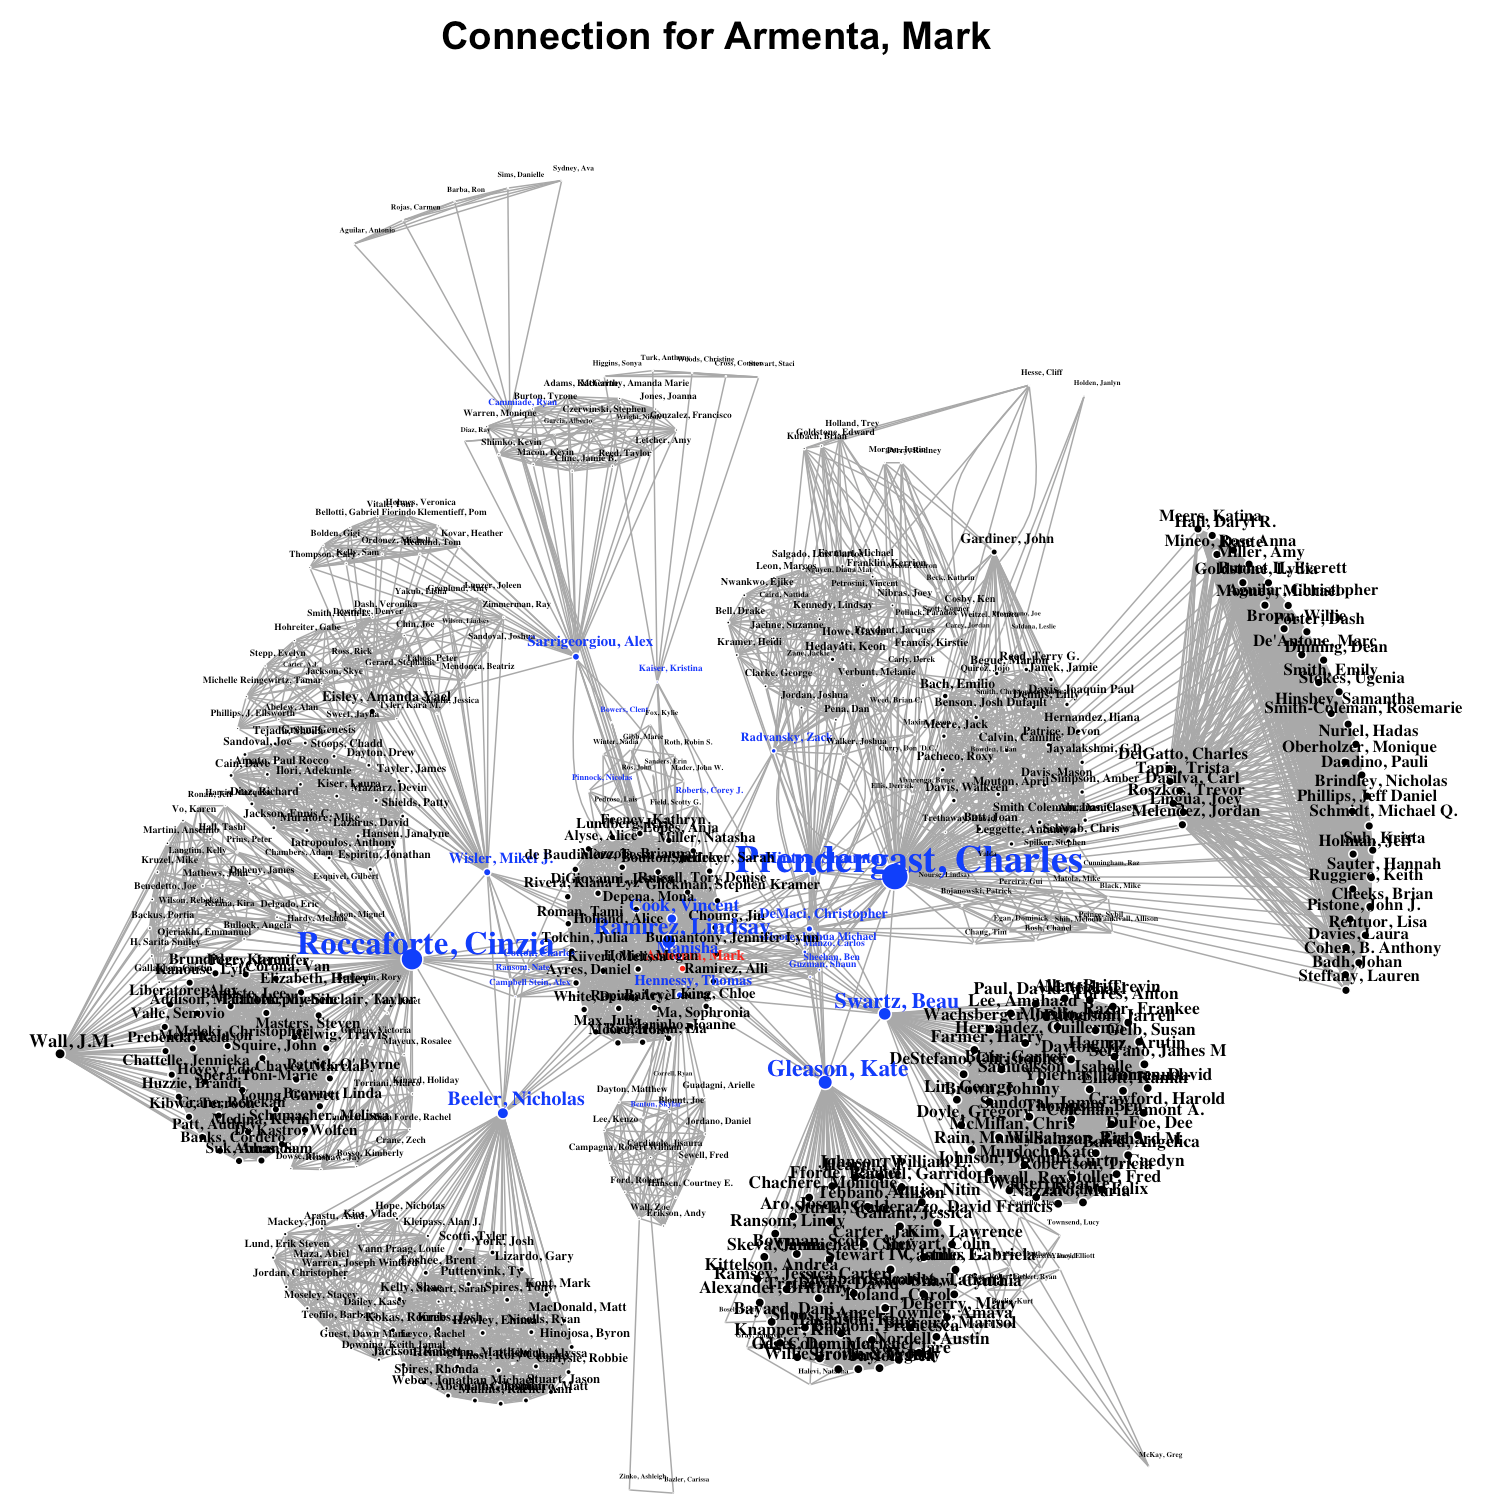
\includegraphics{test2_files/figure-latex/pic2.png}

\begin{Shaded}
\begin{Highlighting}[]
\CommentTok{# For different colors, I note it here: red is for the initial node, blue is the first set of }
\CommentTok{# actors, black is the second set of actors.}
\end{Highlighting}
\end{Shaded}

\subsubsection{14}\label{question-14}

\begin{Shaded}
\begin{Highlighting}[]
\CommentTok{# This is a subquery, since I need the movie stars, I will first select the actors for movies}
\CommentTok{# with nr_order less or equal than 5. Then use these actors to get the final result by }
\CommentTok{# join it to the other tables}
\KeywordTok{dbGetQuery}\NormalTok{(con, }\StringTok{'}
\StringTok{           SELECT title.id, title.title, COUNT(DISTINCT ci.person_id) actor_count}
\StringTok{           FROM title JOIN cast_info ci on title.id = ci.movie_id}
\StringTok{              JOIN (SELECT DISTINCT ci.person_id mvnr_id}
\StringTok{                    FROM title_movie tm JOIN cast_info ci ON tm.id = ci.movie_id}
\StringTok{                    WHERE ci.nr_order IN (1, 2, 3, 4, 5)}
\StringTok{                    ) mvnr ON ci.person_id = mvnr.mvnr_id}
\StringTok{           WHERE ci.role_id IN (1,2)}
\StringTok{              AND title.kind_id = 2}
\StringTok{           GROUP BY ci.movie_id}
\StringTok{           ORDER BY actor_count DESC}
\StringTok{           LIMIT 10}
\StringTok{           '}\NormalTok{)}
\end{Highlighting}
\end{Shaded}

\begin{verbatim}
##         id                     title actor_count
## 1   729678          General Hospital         576
## 2  1404883          One Life to Live         419
## 3   449619         Days of Our Lives         394
## 4   122527             Another World         361
## 5  1941002         The Guiding Light         343
## 6    76799           All My Children         272
## 7   147610        As the World Turns         267
## 8  1970321 The Laurel and Hardy Show         253
## 9  1917967         The Edge of Night         231
## 10 1572213     Retrosexual: The 80's         200
\end{verbatim}

\end{document}
